% !Mode:: "TeX:UTF-8"

\begin{frame}{第二十九讲、Fourier级数}
	\linespread{1.5}
	\begin{enumerate}
	  \item {\bf 内容与要求}{\b (\S 13.2)}
	  \begin{itemize}
		\item 理解Fourier级数的概念
		\item 熟练掌握周期函数的Fourier级数展开
		\item 了解Fourier级数的收敛条件
	  \vspace{1em}
	  \end{itemize}
% 	  \item {\bf  课后作业:}
% 	  \begin{itemize}
% 	    \item {\b 习题13.2:1(1,4),3(1),5,6(3)}
% 	  \end{itemize}
	\end{enumerate}
\end{frame}

\section{三角级数与Fourier级数}

\begin{frame}{函数的局部逼近}
	\linespread{1.2}
	$$\alert{f(x)=\sum\limits_{n=0}^{\infty}\df{f\,^{(n)}(x_0)}{n!}(x-x_0)^n}$$
	\begin{center}
		\resizebox{!}{5cm}{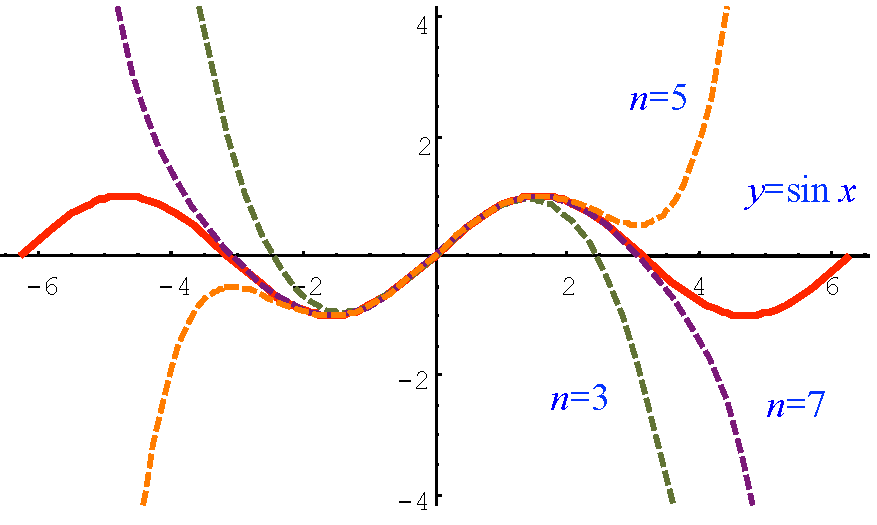
\includegraphics{./images/ch13/sinm.pdf}}
	\end{center}
\end{frame}

% \begin{frame}{最简单的周期运动}
% 	\linespread{1.2} 
% 	{\bb 简谐振动:}例如弹簧振子、钟摆
% 	$$f(t)=A\sin(\omega t+\varphi)$$
% 	\vspace{-1em}
% 	\begin{itemize}
% 	  \item {\b $A$:}振幅 
% 	  \item {\b $\omega$:}角频率 
% 	  \item {\b $\varphi$:}初相位 
% 	\end{itemize}
% 	记$x=\omega t,\,a=A\sin\varphi,\,b=A\cos\varphi$,则
% 	$$\alert{f(x)=a\cos x+b\sin x}$$
% \end{frame}

\begin{frame}{三角级数与周期函数的整体逼近}
	\linespread{1.2}
	\begin{columns}
		\column{.5\textwidth}
			\begin{center}
				\resizebox{!}{3.5cm}{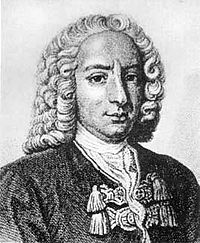
\includegraphics{./images/ch13/db.jpg}}
				
				{\it\small Daniel Bernoulli (1700-1782)}
			\end{center}
			\vspace{-1ex}
			{\b 任何复杂的振动都可以分解成一系列简谐振动之和} 
		\column{.5\textwidth}
			\begin{center}
				\resizebox{!}{3.5cm}{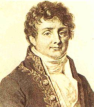
\includegraphics{./images/ch13/fr.pdf}}
				
				{\it\small Joseph Fourier (1768-1830)} 
			\end{center}
			\vspace{-1ex}
			{\b “任意”函数都可以展开成三角级数}\pause 
	\end{columns}
	$$\alert{f(t)=A_0+\sumn A_n\sin(n\omega t+\varphi_n)}$$
\end{frame}

% \begin{frame}{三角级数与周期函数的整体逼近}
% 	\linespread{1.2}\pause 
% 	\begin{columns}
% 		\column{.7\textwidth}
% 			\begin{block}{{\bf Fourier}\hfill}
% 				{\it Any function of a variable, whether continuous or discontinuous, can be
% 				expanded in a series of sines of multiples of the variable.}
% 				
% 				\uncover<3->{\b “任何函数,无论怎样复杂,都可以表示成三角级数的形式。”}
% 			\end{block}
% 		\column{.3\textwidth}
% 			\begin{center}
% 				\resizebox{!}{4cm}{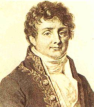
\includegraphics{./images/ch13/fr.pdf}}
% 				
% 				{\it\small Joseph Fourier 
% 				
% 				(1768-1830)}
% 			\end{center}
% 	\end{columns}
% \end{frame}

% \begin{frame}{最简单的周期运动}
% 	\linespread{1.2}\pause 
% 	{\bb 简谐振动:}\pause 例如弹簧振子、钟摆\pause
% 	$$f(t)=A\sin(\omega t+\varphi)$$
% 	\vspace{-1em}
% 	\begin{itemize}\pause 
% 	  \item {\b $A$:}振幅\pause 
% 	  \item {\b $\omega$:}角频率\pause 
% 	  \item {\b $\varphi$:}初相位\pause 
% 	\end{itemize}
% 	记$x=\omega t,\,a=A\sin\varphi,\,b=A\cos\varphi$,\pause 则
% 	$$\alert{f(x)=a\cos x+b\sin x}$$
% \end{frame}

\begin{frame}{三角级数与周期函数的整体逼近}
	\linespread{1.2}
	\vspace{-1em}
	$$\alert{f(x)=\df{\pi}{4}\mathrm{sgn}(x),\;(x\in[-\pi,\pi])
	\;\uncover<2->{\sim\;\sum\limits_{k=1}^n\df{\sin(2k-1)x}{2k-1}}}$$
	\begin{center}
		\only<1-2>{\resizebox{!}{4.8cm}{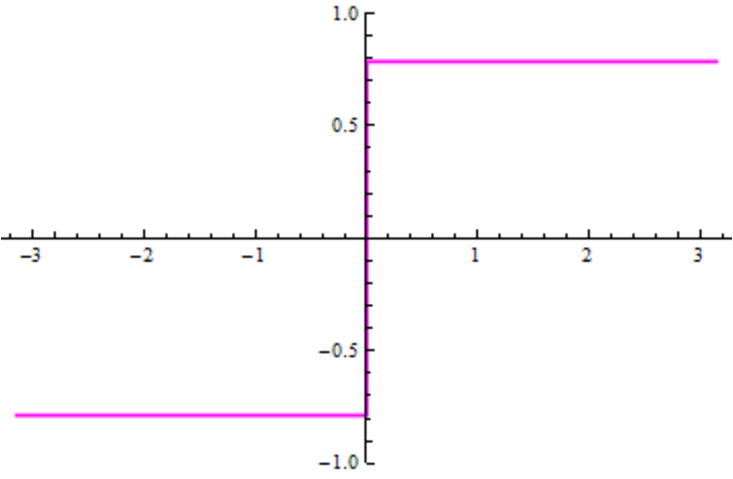
\includegraphics{./images/ch13/fsgn/f0.pdf}}
		
		\invisible<1-2>{$n=0$}}
		\only<3>{\resizebox{!}{4.8cm}{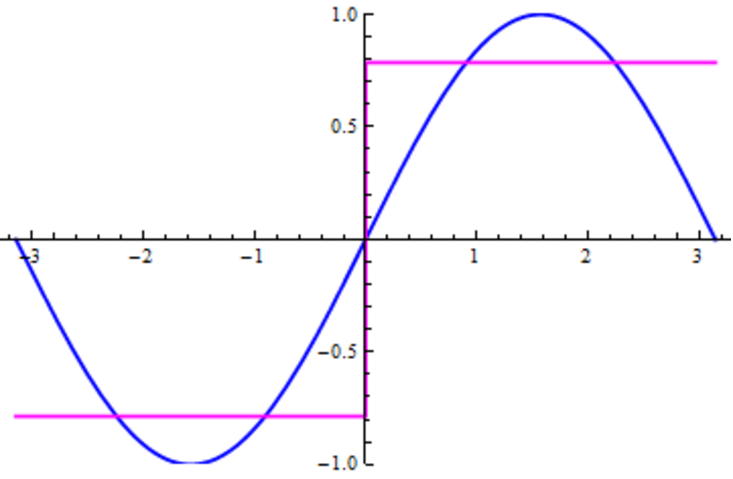
\includegraphics{./images/ch13/fsgn/f1.pdf}}
		
		$n=1$}
		\only<4>{\resizebox{!}{4.8cm}{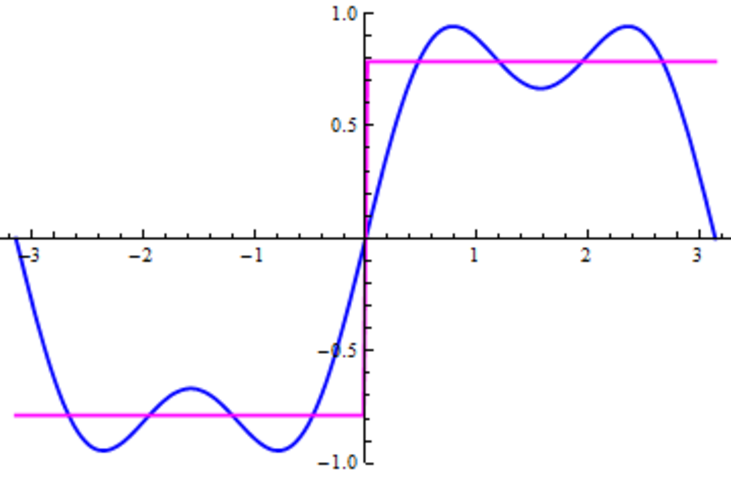
\includegraphics{./images/ch13/fsgn/f2.pdf}}
		
		$n=2$}
		\only<5>{\resizebox{!}{4.8cm}{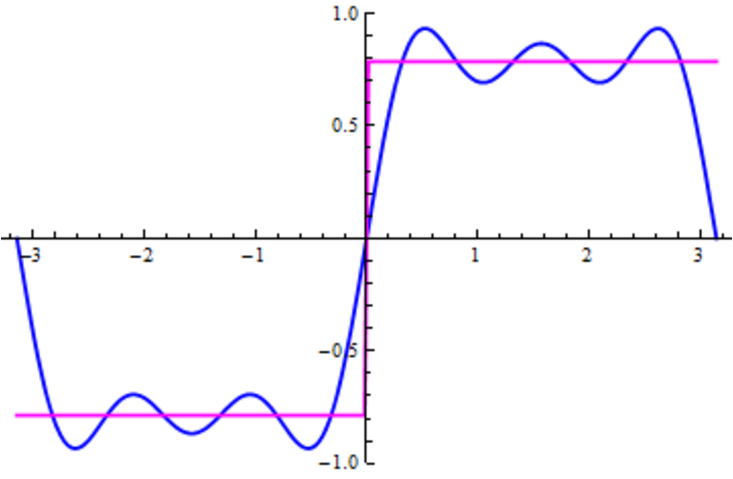
\includegraphics{./images/ch13/fsgn/f3.pdf}}
		
		$n=3$}
		\only<6>{\resizebox{!}{4.8cm}{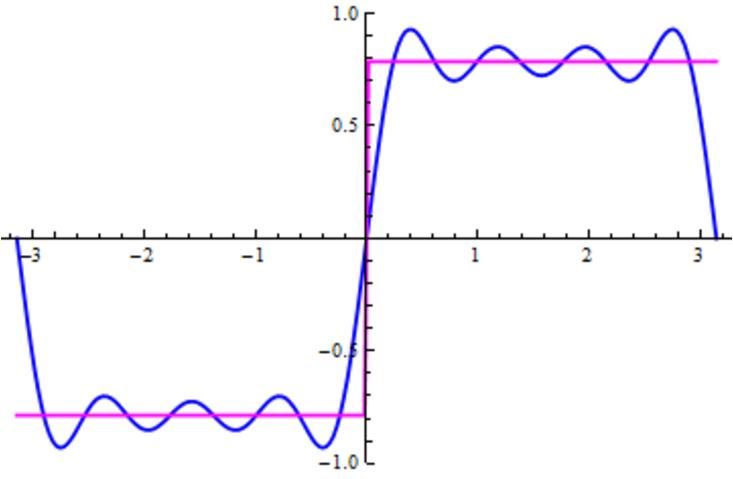
\includegraphics{./images/ch13/fsgn/f4.pdf}}
		
		$n=4$}
		\only<7>{\resizebox{!}{4.8cm}{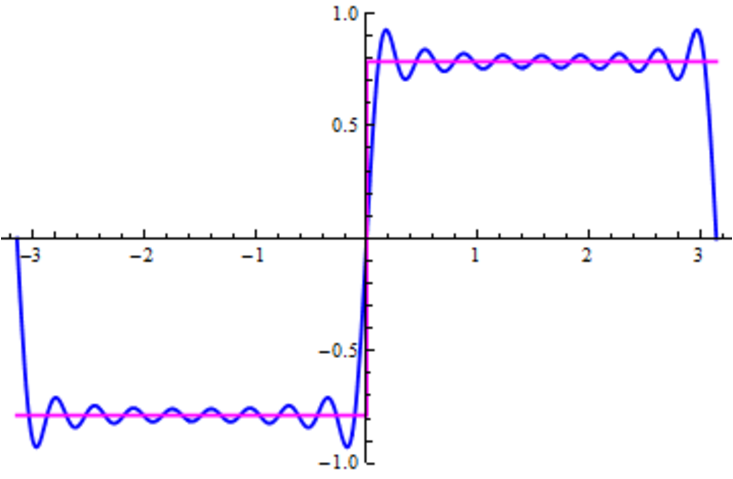
\includegraphics{./images/ch13/fsgn/f5.pdf}}
		
		$n=9$}
	\end{center}
\end{frame}

% \begin{frame}{三角级数}
% 	\linespread{1.2}\pause
% 	$$\alert{\df{a_0}{2}+\sum\limits_{k=1}^{\infty}(a_k\cos kx
% 	+b_k\sin kx)}$$\pause 
% 	\begin{block}{\bf 性质}
% 		三角函数序列$A=\{\cos kx,\sin kx|k=0,1,2,\ldots\}$具有{\bb 正交性}\pause ,
% 		即:任意$f(x),g(x)\in A$,
% 		$$\dint_{-\pi}^{\pi}f(x)g(x)dx=\left\{\begin{array}{ll}
% 		0,\;& f(x)\ne g(x)\\ \pi\;& f(x)=g(x)
% 		\end{array}\right.$$
% 	\end{block}
% \end{frame}

\begin{frame}{Fourier级数}
	\linespread{1.2} 
	\begin{block}{{\bf 定理1}\hfill}
		若函数$f(x)$可展成如下三角级数
		$$\df{a_0}{2}+\sum\limits_{k=1}^{\infty}(a_k\cos kx+b_k\sin kx),$$
		 且{\b 该三角级数可逐项积分}, 则
		$$\left\{\begin{array}{ll}
		a_k=\df1{\pi}\dint_{-\pi}^{\pi}f(x)\cos kxdx,\;& k=0,1,2,\ldots\\[5pt]
		b_k=\df1{\pi}\dint_{-\pi}^{\pi}f(x)\sin kxdx,\;& k=1,2,\ldots
		\end{array}\right.$$
	\end{block}
\end{frame}

% \begin{frame}
% 	\linespread{1.2}
% 	{\bf 注:}
% 	\begin{enumerate}
% % 	  \item 以$2\pi$为周期的三角多项式的Fourier级数是其自身
% % 	  $$\df{a_0}{2}+\sum\limits_{k=1}^{n}(a_k\cos kx+b_k\sin kx)$$
% 	  \item $[-\pi,\pi]$上的奇函数的Fourier级数只含有正弦项,\pause 称为{\bb 正弦级数}
% 	  $$\sum\limits_{k=1}^{n}b_k\sin kx$$\pause 
% 	  \item $[-\pi,\pi]$上的偶函数的Fourier级数只含有余弦项,\pause 称为{\bb 余弦级数}
% 	  $$\df{a_0}{2}+\sum\limits_{k=1}^{n}a_k\cos kx$$
% 	\end{enumerate}
% % 	\begin{exampleblock}{{\bf 例1}\hfill}
% % 		$f(x)$以$2\pi$为周期,且在$[-\pi,\pi]$内$f(x)=\df{\pi}{4}\mathrm{sgn}(x)$,
% % 		求其Fourier级数。
% % 	\end{exampleblock}
% \end{frame}

% \begin{frame}
% 	\linespread{1.2}
% 	\begin{exampleblock}{{\bf 例1}\hfill}
% 		$f(x)$以$2\pi$为周期,且在$[-\pi,\pi]$内$f(x)=\df{\pi}{4}\mathrm{sgn}(x)$,
% 		求其Fourier级数。
% 	\end{exampleblock}\pause 
% % 	\bigskip
% 	\begin{exampleblock}{{\bf 例2}\hfill}
% 		$f(x)$以$2\pi$为周期,且
% 		$$f(x)=\left\{\begin{array}{rl}
% 			-\df{\pi}4,\;& -\pi\leq x<0\\[5pt]
% 			\df{\pi}4,\;& 0\leq x<\pi
% 		\end{array}\right.$$
% 		求其Fourier级数。
% 	\end{exampleblock}\pause 
% 	\begin{itemize}
% 	  \item \alert{只在有限点处取值不同的函数,Fourier级数相同} 
% 	\end{itemize}
% \end{frame}

% \begin{frame}
% 	\linespread{1.2}
% % 	\begin{exampleblock}{{\bf 例1}\hfill}
% % 		$f(x)$以$2\pi$为周期,且在$[-\pi,\pi]$内$f(x)=\df{\pi}{4}\mathrm{sgn}(x)$,
% % 		求其Fourier级数。
% % 	\end{exampleblock}
% % 	\bigskip
% 	\begin{exampleblock}{{\bf 例3}\hfill}
% 		$g(x)$以$2\pi$为周期,且
% 		$$g(x)=\left\{\begin{array}{ll}
% 			0,\;& -\pi\leq x<0\\
% 			1,\;& 0\leq x<\pi
% 		\end{array}\right.$$
% 		求其Fourier级数。
% 	\end{exampleblock}
% \end{frame}

\begin{frame}
	\linespread{1.2}
	\begin{exampleblock}{{\bf 例}\hfill}
		将下列函数展成Fourier级数
		\begin{enumerate}
		  \item $f(x)=1+3\sin x+4\cos 3x-9\sin 2x$\pause
		  \item $f(x)=\sin^4x$\pause
% 		  \item $f(x)=\arcsin(\sin x)$
		\end{enumerate}
	\end{exampleblock}
	\begin{itemize}
	  \item \alert{以$2\pi$为周期的三角多项式的Fourier级数是其自身}
	\end{itemize}
% 	$$\alert{\df{a_0}{2}+\sum\limits_{k=1}^{n}(a_k\cos kx+b_k\sin kx)}$$
\end{frame}

\section{Fourier级数的收敛性}

\begin{frame}{Fourier级数的收敛性}
	\linespread{1.2}\pause 
	\begin{block}{{\bf 定理13.2.1}(Dirichlet收敛条件)\hfill}
		\pause $f(x)$以$2\pi$为周期,\pause 在$[-\pi,\pi]$上其\alert{分段连续}\pause 
		且\alert{仅有有限多个极值点},\pause 则$f(x)$的Fourier级数在$[-\pi,\pi]$上收敛,
		\pause 其和函数
		$$S(x)\pause =\left\{\begin{array}{ll}
			\df{f(x+0)+f(x-0)}{2},\;& x\in(-\pi,\pi)\pause \\[5pt]
			\df{f(-\pi+0)+f(\pi-0)}{2},\;& x=\pm\pi
		\end{array}\right.$$
	\end{block}\pause 
	\begin{itemize}
	  \item {\b $S(x)$在$f(x)$的连续点处收敛于$f(x)$}
% 	  \item {\b 不同函数可能有相同的Fourier级数}
	\end{itemize}
% 	\alert{{\bf 注:}$f(x)$的Fourier级数在其连续点处收敛于$f(x)$}
% 	{\bf 思考:}有哪些函数不满足以上的条件?
\end{frame}

% \begin{frame}
% 	\linespread{1.2}
% 	\begin{exampleblock}{{\bf 例5}\hfill}
% 		试写出函数
% 		$$f(x)=\left\{\begin{array}{rl}
% 			-\df{\pi}{4},\; & -\pi\leq x<0\\[8pt]
% 			\df{\pi}{4},\; & 0\leq x<\pi
% 		\end{array}\right.$$
% 		的Fourier级数的和函数。
% 	\end{exampleblock}
% 	\pause
% 	$$\alert{S(x)=\left\{\begin{array}{ll}
% 		-\pi/4,\;& -\pi<x<0\\
% 		\pi/4,\;& 0<x<\pi\\
% 		0,\; & x=0,\pm\pi
% 	\end{array}\right.}$$
% \end{frame}

\begin{frame}
	\linespread{1.5}
	\begin{exampleblock}{{\bf 例}\hfill}
		设周期函数$f(x)$在一个周期内的表达式为
		$$f(x)=\left\{\begin{array}{ll}
			-1,\;& -\pi<x\leq 0\\
			1+x^2,\; & 0<x\leq\pi
		\end{array}\right.$$
		写出该函数在$[-\pi,\pi]$上的和函数$S(x)$,并求
		$S(5\pi/2),$
		
		$S(7\pi/2),S(7\pi)$和$S(2008\pi)$的值。
	\end{exampleblock}
\end{frame}

% \begin{frame}{利用Fourier级数求特殊级数的和}
% 	\linespread{1.2}\pause 
% 	由
% 	$$\df{\pi}4=\sum\limits_{m=1}^{\infty}
% 	\df{\sin(2m-1)x}{2m-1},\;0<x<\pi,$$
% 	\pause 令$x=\pi/2$,\pause 可得
% 	$$\df{\pi}4=1-\df 13+\df 15-\df 17+\ldots
% 	+(-1)^{m-1}\df 1{2m-1}+\ldots$$
% \end{frame}
% 
% \begin{frame}
% 	\linespread{1.5}
% 	\begin{exampleblock}{{\bf 例7}\hfill}
% 		设$f(x)=|x|\;(-\pi\leq x\leq \pi)$的Fourier级数,并由此
% 		证明:
% 		$$\df{\pi^2}{6}=1+\df 1{2^2}+\df 1{3^2}+\ldots+\df 1{n^2}+\ldots$$
% 	\end{exampleblock}\pause 
% 	$$\alert{|x|=\df{\pi}2-\df 4{\pi}\sum\limits_{m=1}^{\infty} 
% 	\df{\cos(2m-1)x}{(2m-1)^2},\;-\pi\leq x\leq \pi}$$
% \end{frame}

\begin{frame}
	\linespread{1.5}
	\begin{exampleblock}{{\bf 思考}\hfill}
		设周期函数$f(x)$在一个周期内的表达式为
		$$f(x)=e^x\;(x\in[0,2\pi]),$$
		试将其展成Fourier级数,并求下列数值级数的和:
		$$\sum\limits_{n=1}^{\infty}\df1{1+n^2}$$
	\end{exampleblock}
\end{frame}

\section{函数的延拓及其Fourier展开}

\begin{frame}{函数的延拓及其Fourier展开}
	\linespread{1.3}\pause 
	{{\bf 问题:}如果函数$f(x)$只在$(0,\pi)$或$[0,\pi]$上有定义,能否/如何对其进行
	Fourier展开?}\pause 
	
	\bigskip
	\ba{函数(定义)的延拓:}\pause 扩充函数的定义域,使其具有某种期望的性质\pause 
	\begin{enumerate}
	  \item {\b 周期延拓:}\pause 延拓后为周期函数\pause 
	  \item {\b 奇延拓:}\pause 延拓后为奇函数\pause 
	  \item {\b 偶延拓:}\pause 延拓后为偶函数
	\end{enumerate}	
\end{frame}

% \begin{frame}{1、周期延拓}
% 	\linespread{1.2}\pause 
% 	设$f(x)$在$(0,\pi)$上满足Dirichlet条件\pause 
% 	\begin{enumerate}
% 	  \item 任取在$[-\pi,0]$上满足Dirichlet条件的函数$g(x)$\pause 
% 	  \item 令
% 	  $$F(x)=\left\{\begin{array}{ll}
% 	  	f(x),\;& x\in(0,\pi)\\
% 	  	g(x),\;& x\in[-\pi,0]
% 	  \end{array}\right.$$
% 	  \pause 且
% 	  $$F(x+2\pi)=F(x)\;(-\infty<x<\infty)$$
% 	\end{enumerate}
% 	\pause \ba{$F(x)$为$(-\infty,\infty)$上满足Dirichlet条件的周期函数,
% 	其在$(0,\pi)$上$f(x)$有相同的Fourier展开式}
% \end{frame}
% 
% \begin{frame}{2、奇(性)延拓}
% 	\linespread{1.2}\pause 
% 	设$f(x)$在$(0,\pi)$上满足Dirichlet条件\pause 
% 	\begin{itemize}
% % 	  \item 任取在$[-\pi,0]$上满足Dirichlet条件的函数$g(x)$
% 	  \item 令
% 	  $$F(x)=\left\{\begin{array}{ll}
% 	  	f(x),\;& x\in(0,\pi)\\
% 	  	0,\;& x=0,-\pi\\
% 	  	-f(-x),\;& x\in(-\pi,0)
% 	  \end{array}\right.$$
% 	  \pause 且
% 	  $$F(x+2\pi)=F(x)\;(-\infty<x<\infty)$$
% 	\end{itemize}
% 	\pause \ba{$F(x)$为满足Dirichlet条件的奇周期函数,其Fourier级数为正弦级数,且
% 	在$(0,\pi)$内与$f(x)$的展式相同}
% \end{frame}
% 
% \begin{frame}{3、偶(性)延拓}
% 	\linespread{1.2}\pause 
% 	设$f(x)$在$[0,\pi]$上满足Dirichlet条件\pause 
% 	\begin{itemize}
% % 	  \item 任取在$[-\pi,0]$上满足Dirichlet条件的函数$g(x)$
% 	  \item 令
% 	  $$F(x)=\left\{\begin{array}{ll}
% 	  	f(x),\;& x\in[0,\pi]\\
% 	  	f(-x),\;& x\in[-\pi,0)
% 	  \end{array}\right.$$
% 	  \pause 且
% 	  $$F(x+2\pi)=F(x)\;(-\infty<x<\infty)$$
% 	\end{itemize}
% 	\pause \ba{$F(x)$为满足Dirichlet条件的偶周期函数,其Fourier级数为余弦级数,且
% 	在$(0,\pi)$内与$f(x)$的展式相同}
% \end{frame}

\begin{frame}
	\linespread{1.2}
	\begin{exampleblock}{{\bf 例}\hfill}
		设函数$f(x)=x+1\,(x\in(0,\pi))$,试将其分别展开为正弦和余弦级数。\pause 
	\end{exampleblock}
	\begin{center}
		\resizebox{!}{2.7cm}{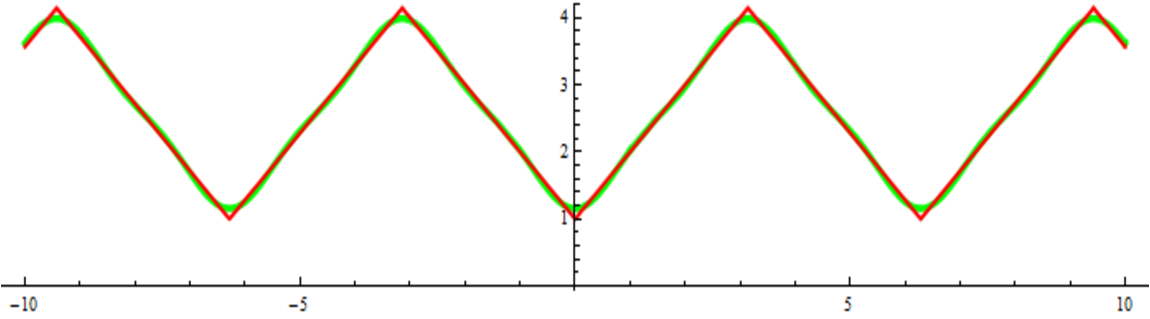
\includegraphics{./images/ch13/cs.pdf}}\pause 
		
		\resizebox{!}{2.7cm}{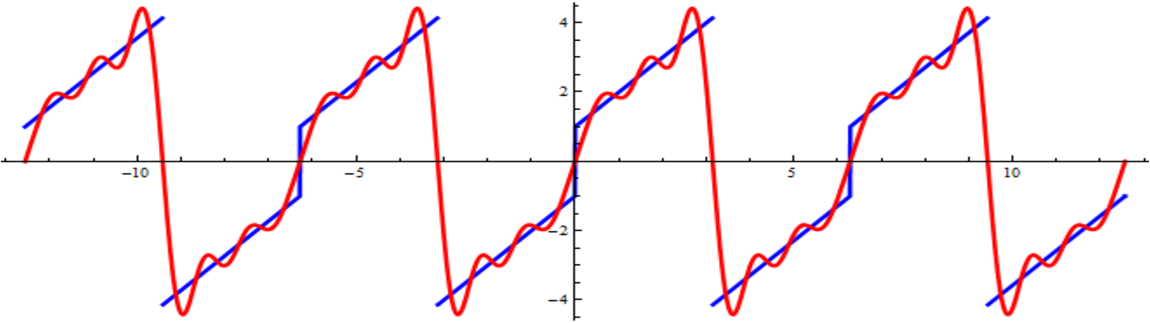
\includegraphics{./images/ch13/ss.pdf}}
	\end{center}
\end{frame}

\begin{frame}
	\linespread{1.2}
	\begin{exampleblock}{{\bf 例}\hfill}
		设$f(x)=\pi x-x^2\,(0<x<\pi)$,又设$S(x)$是$f(x)$在$(0,\pi)$内以
		$2\pi$为周期的正弦级数展开式的和函数,求当$x\in(\pi,2\pi)$时$S(x)$的表达式。
	\end{exampleblock}
\end{frame}

\section{周期为$2l$的Fourier级数}

\begin{frame}{周期为$2l$的Fourier级数}
	\linespread{1.4}\pause 
	{\bf 问题:}对周期为$2l\ne2\pi$的函数$f(x)$,能否/如何将其展开为Fourier级数?\pause 
	
	\alert{\bf 伸缩变换:}\pause 令$t=\df{\pi}{l}x$,\pause
	则$g(t)=f\left(\df{l}{\pi}t\right)$ 是以$2\pi$为周期的函数。\pause 
	对$g(t)$做Fourier展开,由其展开式可变换得到$f(x)$的展开式。\pause 
	
	\bigskip
	\begin{exampleblock}{{\bf 例11}\hfill}
		将函数$f(x)=x\,(0<x<1)$表示为只有余弦项的三角级数。
	\end{exampleblock}
\end{frame}

\begin{frame}[<+->]{小结}
	\linespread{1.5}
	\begin{enumerate}
	  \item {\bf 三角级数:}正交函数序列
	  \item {\bf Fourier级数}
	  \begin{itemize}
	    \item Fourier系数
	    \item Dirichlet收敛条件
	    \item 正(余)弦级数
	  \end{itemize}
	  \item 函数的定义延拓与Fourier展开
	  \item 周期为$2l$的函数的Fourier展开
	\end{enumerate}
\end{frame}

\begin{frame}{判断正误}
	\linespread{1.5}\pause 
	\begin{enumerate}
	  \item 函数$f(x)$连续,在$[-\pi,\pi]$上满足Dirichlet条件且为奇函数,则$f(x)$
	  的Fourier级数在$0,\pm\pi$处必收敛于$0$\pause\quad  (\;\alert{$\surd$}\;)\pause 
	  \item $f(x)=x^2\,(x\in[-\pi,\pi])$的Fourier级数在$2\pi$处收敛于$4\pi^2$
	  \pause  \quad(\;\alert{$\times$}\;)\pause 
	  \item 以$2\pi$为周期的函数$f(x)=\df x{2\pi}\,(x\in[0,2\pi])$,其Fourier
	  级数的和函数为$S(x)$,则$S(0)=f(0)=0$
	  
	  \pause\quad (\;\alert{$\times$}\;)
	\end{enumerate}
\end{frame}

\begin{frame}{判断正误}
	\linespread{1.5}
	\begin{enumerate}
	  \addtocounter{enumi}{3}
	  \item 函数$f(x)=x^2\,(x\in[-\pi,\pi])$以$2\pi$为周期,则\pause 
	  \begin{itemize}
	    \item $\df 1{\pi}\dint_{-\pi}^{\pi}f(x)\sin kxdx=\df
	    1{\pi}\dint_{0}^{2\pi}f(x)\sin kxdx$\pause\quad (\;\alert{$\surd$}\;)\pause 
	    \item $\df 1{\pi}\dint_{-\pi}^{\pi}x^2\sin kxdx=\df
	    1{\pi}\dint_{0}^{2\pi}x^2\sin kxdx$\pause\quad (\;\alert{$\times$}\;)\pause 
	  \end{itemize}
	  \item 以$2\pi$为周期的函数$f(x)=x^2\,(x\in[-\pi,\pi])$和$g(x)=x^2\,(x\in[0,2\pi])$的
	  Fourier级数相同\pause\quad (\;\alert{$\times$}\;)
	\end{enumerate}
\end{frame}

\begin{frame}
	\linespread{1.2}
	\begin{exampleblock}{{\bf 例12}\hfill}
		将下列函数展成Fourier级数
		\begin{enumerate}
% 		  \item $f(x)=x-[x]$
		  \item $f(x)=\sin^4x$
		  \item $f(x)=\arcsin(\sin x)$
		\end{enumerate}
	\end{exampleblock}
\end{frame}

\begin{frame}
	\linespread{1.2}
	\begin{exampleblock}{{\bf 例13}\hfill}
		设$f(x)$是以$2\pi$为周期的连续函数,在$[-\pi,\pi]$上满足Dirichlet条件,
		且其Fourier系数为$a_k,b_k$。设
		$$G(x)=\df1{\pi}\dint_{-\pi}^{\pi}f(t)f(x+t)dt$$
		\vspace{-1em}
		\begin{enumerate}
		  \item 证明$G(x)$为偶函数
		  \item 求$G(x)$的Fourier系数
		  \item 证明$\df1{\pi}\dint_{-\pi}^{\pi}f\,^2(x)dx=\df{a_0^2}2+
		  \sum\limits_{k=1}^{\infty}(a_k^2+b_k^2)$
		\end{enumerate}
	\end{exampleblock}
\end{frame}

%=====================================

% \begin{frame}{title}
% 	\linespread{1.2}
% 	\begin{exampleblock}{{\bf title}\hfill}
% 		123
% 	\end{exampleblock}
% \end{frame}
% 
% \begin{frame}{title}
% 	\linespread{1.2}
% 	\begin{block}{{\bf title}\hfill}
% 		123
% 	\end{block}
% \end{frame}